\chapter{Weryfikacja rozwiązania}

W celu weryfikacji poprawności działania zaiplementowanego systemu zostały
wykonane serie testów. System został przetestowany pod kątem sprawdzenia
podstawowych założeń projektowych tj. poprawności wykrywania anomali, związanych
z natężeniem ruchu, w obsługiwanej sieci oraz możliwości skalowania
aplikacji \textit{sdn\_epc} w celu zwiększenia wydjaności systemu.
Przeprowadzenie testów wymagało przygotowania odpowiednich scenariuszy testowych,
zestawienia dedykowanych topolgi sieciowych oraz stworzenia rozwiązań
pozwalających na zebranie własciwych danych z testowanego systemu. Analiza
tychże wyników pozwoliła na stwierdzenie, czy i w jakim stopniu założenia
projektowe zostały spełnione. Niniejszy rozdział szczegółowo opisuje
poszczególne przypadki testowe oraz prezentuje analizę uzyskanych wyników.

\section{Test działania implementacji algorytmu}

% w jaki sposób sprawdzamy czy algorytm działa? Liczymy entropie, trzeba to
% ująć
 
Aby stwierdzić, czy zaimplementowany algorytm (\pageref{equ:entropy}) w aplikacji
\textit{sdn\_epc} spełnia swoją rolę tzn. pozwala wykryć atak DDoS w sieci SDN
zostały przeanalizowane wartości entropii obliczone za pomocą tegoż właśnie
algorytmu w dwóch różnych przypadkach testowych, z których każdy wykorzystywał
nieco inną konfigurację testową topologi sieciowej, jak również samej aplikacji
\textit{sdn\_epc}. Przetestowane zostały przypadki, gdy: 
\begin{enumerate}
  \item Ruch wygenerowany w sieci testowej był obsługiwany tylko przez jeden
    węzeł aplikacji \textit{sdn\_epc}.
  \item Ruch wygenerowanych w sieci testowej był obsługiwany przez wiele węzłów
    aplikacji \textit{sdn\_epc} działających w klastrze.
\end{enumerate}
Wykorzystanie takich właśnie przypadków testowych umożliwiło sprawdzenie
poprawności implementacji algorytmu zarówno w przypadku działania systemu jako
pojedynczy węzeł aplikacji \textit{sdn\_epc}, jak również w przypadku, gdy
system działał w klastrze. Drugi przypadek jest znacznie bardziej złożony,
ponieważ rozproszenie procesu obliczania algorytmu na wiele węzłów wprowadza
dodatkowe komplikacje, związane z synchronizacją stanu pomiędzy węzłami w
klastrze.

\subsection{Przypadek testowy z wykorzystaniem jednego węzła aplikacji
  \textit{sdn\_epc}}

Schemat topologii sieciowej, wykorzystanej w przypadku, gdy tylko jeden węzeł
aplikacji jest zaangażowany w przetwarzenie ruchu został przedstawiony na
Rys. \ref{fig:entropia_scheme}.

\begin{figure}[h]
\centering
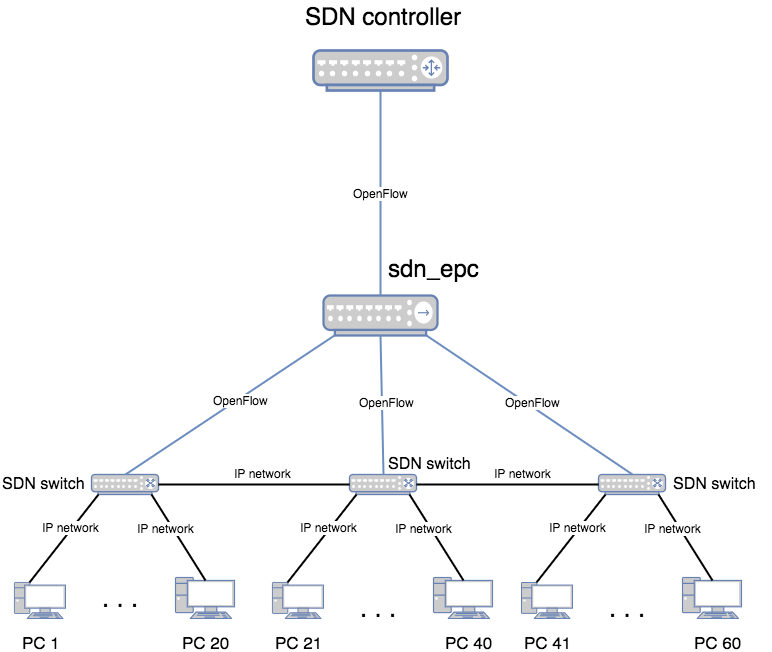
\includegraphics[width=\textwidth]{entropia_scheme}
\caption{Schemat topologii sieciowej z wykorzystaniem jednego węzła aplikacji
  \textit{sdn\_epc}}
\label{fig:entropia_scheme}
\end{figure}

W topologii przedstawionej na Rys. \ref{fig:entropia_scheme} wszystkie
przełączniki obsługujące ruch pomiędzy węzłami końcowymi (\textit{PC N})
komunikują się z kontrolerem (\textit{SDN controller}) poprzez jeden węzeł
aplikacji \textit{sdn\_epc}. Wykorzystując taką konfigurację sieci, tylko jeden
węzeł \textit{sdn\_epc} przetwarza wiadomości \mbox{\textit{PACKET\_IN}}
protokołu \textit{OpenFlow}, wymieniane pomiędzy poszczególnymi przełącznikami,
a kontrolerem, w celu obliczenia entropii pakietów przesyłanych w sieci.

Jeśli algorytm został poprawnie zaimplementowany to wartość entropii,
obliczonej za jego pomocą, powinna maleć wzraz ze spadkiem losowości pakietów
przesyłanych w sieci testowej. Innymi słowy, im więcej pakietów w sieci jest
adresowanych do pojedynczego węzła końcowego, tym mniejsza będzie wartość
obliczonej entropii.

W celu sprawdzenia czy wspomiana zależność została spełniona, koniecznym było
zaprojektowanie odpowiedniego scenariusza testowego. Scenariusz ten opierał się
na środowisku testowym przedstawionym na Rys. \ref{fig:entropia_tech}.

\begin{figure}[h]
\centering
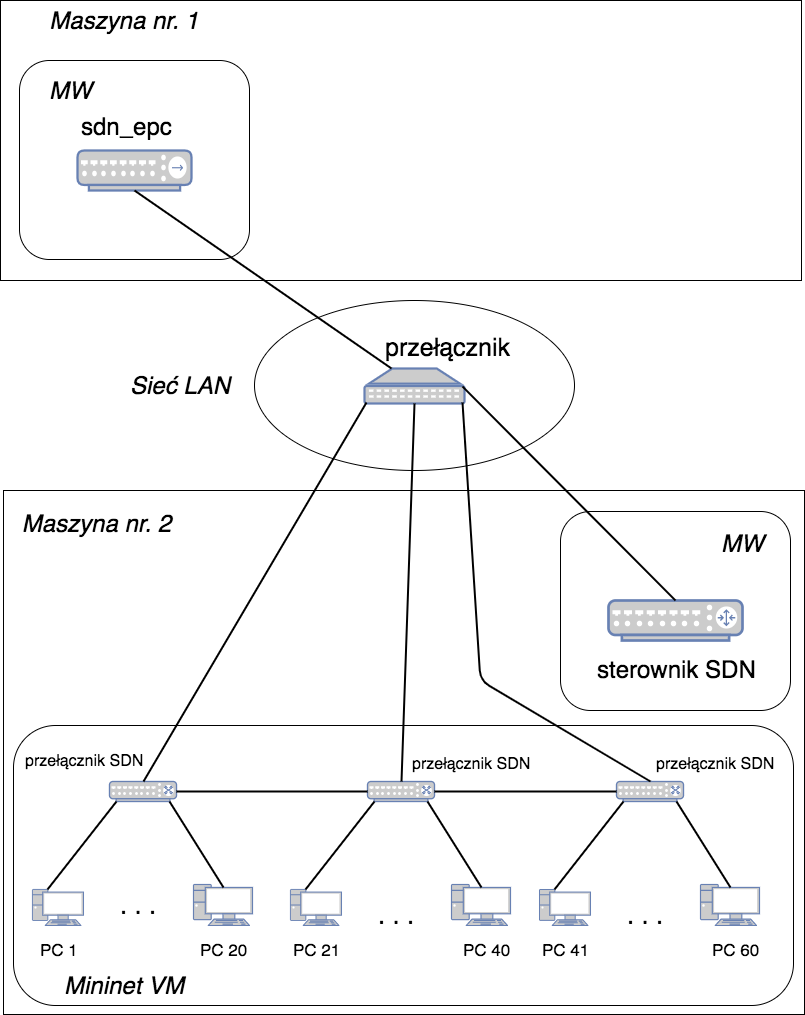
\includegraphics[height=11cm]{entropia_tech}
\caption{Środowisko testowe z wykorzystaniem jednego węzła aplikacji
  \textit{sdn\_epc}}
\label{fig:entropia_tech}
\end{figure}

Jak przedstawiono na Rys. \ref{fig:entropia_tech} toplogia sieciowa została
zestawiona z użyciem dwóch maszyn fizycznych, na których zostały zwirtualizowane
niezbędne komponenty testowe. Każdy z komponentów, za wyjątkiem przełącznika
sieci \textit{LAN} (\textit{switch}), został uruchomiony na dedykowanej maszynie
wirtualnej. Jako środowisko do wirtualizacji zostało wykorzystane oprogramowanie
\textit{VirtualBox \footnote{https://www.virtualbox.org}}. Maszyny wirtualne
komunikowały się ze sobą z wykorzystaniem sieci \textit{LAN}.

Przełączniki sieci SDN (\textit{SDN switch}'es) oraz węzły końcowe (\textit{PC
  N}) były emulowane na dedykowanej maszynie wirtualnej za pomocą oprogramowania
\textit{Mininet \footnote{http://mininet.org}}. Wykorzystane w teście
przełączniki to domyślne przełączniki używane przez oprogramowanie
\textit{Mininet}, które działają na bazie oprogramowania
\textit{Open vSwitch \footnote{http://openvswitch.org}}.
\textit{SDN controller}, pełniący funkcję kontrolera w testowej topologii,
korzystał z oprogramowania zbudowanego z wykrzystaniem framework'a
\textit{Ryu \footnote{https://osrg.github.io/ryu}}. Maszyny wirtualne dedykowane
dla \textit{sdn\_epc} i \textit{SDN controller} działały pod kontrolą systemu
operacyjnego \textit{Ubuntu \footnote{https://www.ubuntu.com}}.

Scenariusz testowy zakładał przeprowadzenie kilku prób, podczas których w sieci
były generowane ataki DDoS o różnej sile. Podczas każdej próby została zmierzona
średnia wartość entropii obliczonej za pomocą zaimplementowanego algorytmu.
Wykonane zostały cztery próby z atakami o sile odpowiednio: 0\%, 30\%, 60\% oraz
90\%. Siła każdego ataku została obliczona na podstawie wzoru
\ref{equ:ddos_power}

\begin{equation}
R = \frac{P_{a}}{P_{n}} \cdot 100\%
\label{equ:ddos_power}
\end{equation}
gdzie R oznacza siłę ataku, $P_{a}$ pakiety atakujące, natomiast $P_{n}$ pakiety
tła.

Pakiety tła rozumiane są jako pakiety
\textit{IP \footnote{https://tools.ietf.org/html/rfc791\#section-3.1}} wysyłane
do losowo wybranych węzłów końcowych w stałych odstępach czasowych. Pakiety
atakujące oznaczają pakiety \textit{IP}, które zawierają losowe adresy docelowe
oraz są wysyłane do konkretnego węzła końcowego w 4-krotnie krótszych odstępach
czasowych niż pakiety tła. 

Podczas każdej próby wybrane węzły końcowe generowały pakiety tła oraz
pakiety atakujące (jeden węzeł generował jeden typ pakietów). Do generowania
pakietów została wykorzystana biblioteka języka \textit{Python} o nazwie
\textit{ Scapy \footnote{http://www.secdev.org/projects/scapy}}. Szczegółowe
dane opisujące każdą z prób zostały przedstawione w tab. \ref{tab:entropy}.
\newpage

\begin{table}[h!]
\centering
\begin{tabular}{ |c|c|c|c|c| } 
 \hline
 R & $P_{n}$ & $P_{a}$ & interwał $P_{n}$ & interwał $P_{a}$ \\
 \hline
 0\% & 3000 & 0 & 20ms & 5ms \\ 
 \hline
 30\% & 3000 & 900 & 20ms & 5ms \\ 
 \hline
 60\% & 3000 & 1800 & 20ms & 5ms \\ 
 \hline
 90\% & 3000 & 2700 & 20ms & 5ms \\ 
 \hline
\end{tabular}
\caption{Parametry prób testowych z wykorzystaniem jednego węzła aplikacji
  \textit{sdn\_epc}} 
\label{tab:entropy}
\end{table}

Warto zaznaczyć, że średnio 3,4\% wszystkich pakietów z danej próby nie dotarło
do aplikacji \textit{sdn\_epc}. Wydaje się, że nie powinno wpływać to znacząco
na uzyskane wyniki, jednak, ze względu na fakt, że przeprowadzenie tego typu
testów wymaga znaczących zasobów obliczeniowych, do których dostęp nie jest
ogólnodostępny, wpływ wspomianego zjawiska nie został naukowo zbadany.

Na wykresie \ref{plot:entropy} przedstawiono średnią wartość entropii,
obliczonej przez aplikację \textit{sdn\_epc} przy użyciu zaimplementowanego w
niej algorytmu, dla poszczególnych prób testowych.

\begin{figure}[h]
\centering
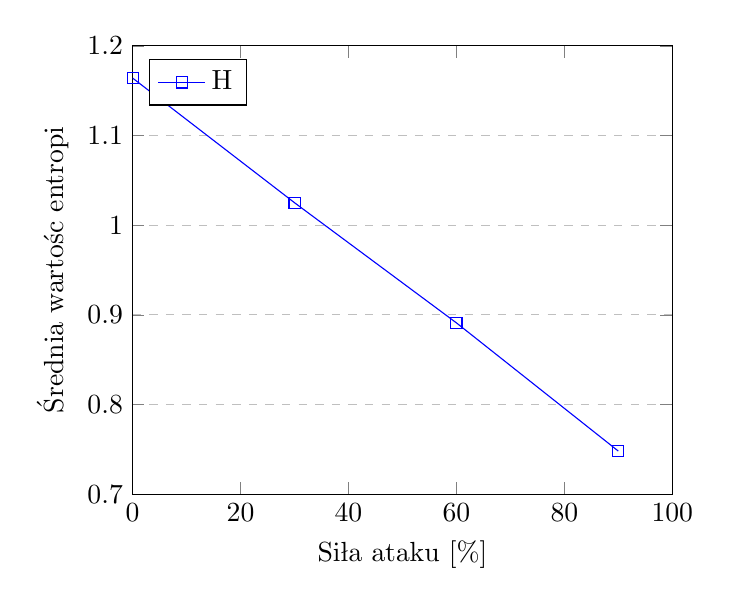
\begin{tikzpicture}
\begin{axis}[
    xlabel={Siła ataku [\%]},
    ylabel={Średnia wartośc entropi},
    xmin=0, xmax=100,
    ymin=0.7, ymax=1.2,
    xtick={0,20,40,60,80,100},
    ytick={0.7,0.8,0.9,1,1.1,1.2},
    legend pos=north west,
    ymajorgrids=true,
    grid style=dashed,
]
 
\addplot[
    color=blue,
    mark=square,
    ]
    coordinates {
    (0,1.164)(30,1.025)(60,0.891)(90,0.748)
    };
    \legend{H}
 
\end{axis}
\end{tikzpicture}
\caption{Średnia wartość entropii w zależności od siły ataku DDoS}
\label{plot:entropy}
\end{figure}

Zależność entropii od siły ataku, przedstawiona na wykresie \ref{plot:entropy},
jest taka, jak przewidywano. Wzraz ze wzorstem siły ataku wartość entropii
maleje, ponieważ im większa siła ataku, tym większy procent wszystkich pakietów
w sieci trafia do jednego, atakowanego, węzła końcowego. W związku z tym,
losowość poszczególnych pakietów spada, tym samym powodując spadek entropii
pakietów w sieci.

Bazując na przestawionych wynikach i ich analizie, można stwiedzić, że alogorytm
służacy do wykrywania ataku DDoS, został poprawnie zaimplementowany w aplikacji
\textit{sdn\_epc} i umożliwa wykrycie tego typu anomali. 
